\documentclass{article}
\usepackage{fullpage}
\usepackage[]{amsmath}
\usepackage[]{siunitx}
\usepackage[]{gensymb}
\usepackage[]{steinmetz}
\usepackage[]{chngcntr}
\usepackage[]{dsfont}
\usepackage[]{hyperref}
\usepackage[]{xcolor}
\usepackage[final]{pdfpages}
\hypersetup{
    colorlinks,
    linkcolor={blue!50!black},
    citecolor={blue!50!black}
}
\numberwithin{equation}{section}
\renewcommand{\thesection}{}
\renewcommand{\thesubsection}{}
\renewcommand{\thesubsubsection}{}
\renewcommand{\theequation}{\thesection\arabic{equation}}
\makeatletter
\def\@seccntformat#1{\csname #1ignore\expandafter\endcsname\csname the#1\endcsname\quad}
\let\sectionignore\@gobbletwo
\let\latex@numberline\numberline
\def\numberline#1{\if\relax#1\relax\else\latex@numberline{#1}\fi}
\makeatother
\title{ECE 671 Fall 2015 Assignment 3}
\author{John Rinehart}
\date{\today}

\begin{document}
\maketitle
\tableofcontents
\section*{Foreword}

This problem set had me using a few tools at different times. I used Keysight's
Advanced Design Suite (ADS) at a few points during my homework, for simulations.
I have also used Mathematica, extensively, to assist me with algebra and
plugging in values. Each problem is more or less self-contained in the written
text. However, if you want to see calculations or simulations of anything that
is referenced in the problem please consult the appendix for the associated
problem. I have almost as many appendices as problems to account for this extra
information. Please don't hesitate to ask me any questions you may have
concerning my work. I have done my best to make it clear, but sometimes clear is
only ``clear'' to one's self.

\section*{Problem 1a}
The maximum power available from the source is determined by the condition where
the source is conjugately matched to the load (this is when $Z_s = Z_{in}^*$).
The load impedance is specified as 100~$\Omega$. Thus, a conjugately matched
input impedance would be given by (100~$\Omega$)$^*$. This load will divide the
voltage of the source. Thus, the power available
from the source is given by:
\begin{align*}
    P_{avl} &= \Re(V_{in}I_{in}^*) \\
            &= \Re(\frac{|V_{in}|^2}{Z_{in}^2} \\
            &= \Re\left(\frac{(\SI{10}{\volt)^2}}{100 \Omega}\right) \\
            &= \SI{1}{\watt}
\end{align*}
\section*{Problem 1b}
\subsection*{Port 1 Waves}
To calculate the port 1 power waves I will use the following 
relationships:
\begin{align}
    \sqrt{Z_c}\left( a_1 + b_1 \right) &= V_s \frac{Z_{in}}{Z_{in}+Z_s}
    \label{eq1} \\
    b_1 &= \Gamma_{in}a_1 \label{eq2} \\
    \Gamma_{in} &=\frac{Z_{in}-Z_c}{Z_{in}+Z_c} \label{eq3}
\end{align}
Combining (\ref{eq1}) and (\ref{eq2}) yields:

\begin{equation}
    a_1 = \frac{V_s}{\sqrt{Z_c}} \frac{1}{( 1+\Gamma_{in} )}
    \frac{Z_{in}}{Z_{in}+Z_s} \label{prea1}
\end{equation}

Rearranging (\ref{eq3}) for $Z_{in}$ produces $Z_{in} = Z_c
\frac{1+\Gamma_{ in }}{1-\Gamma_{ in }}$. Substituting this into (\ref{prea1}) yields:

\begin{align}
    a_1 &= \frac{V_s}{\sqrt{Z_c}( 1+\Gamma_{in} )} \frac{Z_c \frac{1+\Gamma_{ in }}{1-\Gamma_{
    in }}}{Z_c \frac{1+\Gamma_{ in }}{1-\Gamma_{ in }} + Z_s} \nonumber \\
    &= \frac{V_s}{\sqrt{Z_c}( 1+\Gamma_{in} )} \frac{Z_c \left( 1+\Gamma_{in}
    \right)}{Z_c \left( 1+ \Gamma_{in} \right) + Z_s \left( 1 - \Gamma_{in}
    \right)} \nonumber \\
    &= V_s \frac{\sqrt{Z_c}}{Z_c \left( 1+\Gamma_{in} \right) + Z_s \left( 1 -
\Gamma_{in} \right) } \label{a1}
\end{align}

$b_1$ is easily obtained from this using (\ref{eq2}). 
\begin{equation}        
b_1 = V_s \frac{\sqrt{Z_c}\Gamma_{in}}{Z_c \left( 1+\Gamma_{in} \right) +
Z_s(1-\Gamma_{in})} \label{b1}
\end{equation}

Notice that if $\Gamma_{in} = 1$ (an open) that 
$a_1 = \frac{V_s}{2 \sqrt{Z_c}}$
and 
$b_1 = \frac{V_s}{2 \sqrt{Z_c}}$ such
that 
$V_{load} = \sqrt{Z_c} (a_1+b_1) = V_s$ (reflects completely in phase).

If $\Gamma_{in} = -1$ (a short)
\begin{gather*}
    a_1 = \frac{V_s \sqrt{Z_c}}{2 Z_s} \\
    b_1 = -\frac{V_s\sqrt{Z_c}}{2Z_s} \\
    V_{load} = 0
\end{gather*}

If $\Gamma_{in} = 0$ (a matched load)
\begin{gather*}
    b_1 = 0 \\
    a_1 = \frac{V_s \sqrt{Z_c}}{Z_c + Z_s} \\
    V_{load} = \frac{V_s Z_c}{Z_c + Z_s}
\end{gather*}

But, of course, in matched conditions $Z_c = Z_L$.
\subsection*{Port 2 Waves}
Calculating the port 2 power waves I will use the following relationships:

\begin{align}
    b_2 &= S_{21}a_1 + S_{22}a_2 \label{eq1a}\\
    a_2 &= \Gamma_l b_2 \label{eq2a} \\
    a_1 &= V_s \frac{\sqrt{Z_c}}{Z_c \left( 1+\Gamma_{in} \right) + Z_s \left( 1 -
\Gamma_{in} \right)} \label{eq3a}
\end{align}

Combining (\ref{eq1a}) and (\ref{eq2a}) yield:

\begin{equation}
b_2 = \frac{S_{21}a_1}{1-S_{22}\Gamma_l} \label{eq4a}
\end{equation}

Combining (\ref{eq4a}) and (\ref{eq3a}) yields:

\begin{equation}
    b_2 =  \frac{V_s \sqrt{Z_c}}{Z_c \left( 1 + \Gamma_{in} \right) +
    Z_s(1-\Gamma_{in})}\frac{S_{21}}{1-S_{22}\Gamma_l} \label{b2}
\end{equation}

Obtaining $a_2$ from (\ref{eq2a}) and (\ref{eq5a}) is trivial:

\begin{equation}
    a_2 = \frac{V_s \sqrt{Z_c}}{Z_c \left( 1+\Gamma_{in} \right) +
    Z_s(1-\Gamma_{in})}\frac{S_{21}\Gamma_l}{1-S_{22}\Gamma_l} \label{a2}
\end{equation}
%TODO: DEFINE AND GAMMA_IN
\section*{Problem 1c}
To determine the power delivered to the load we begin with the definition of
real power

\[ 
        P_{load} =  \frac{1}{2}\Re\left( V_{load}I^*_{load} \right) 
\]

In this case, $V_{load} = \sqrt{Z_c} \left( a_2 + b_2 \right) $ and $I_{load} =
\frac{b_2-a_2}{\sqrt{Z_c}}$. But, $a_2 = b_2 \Gamma_l$ so $P_{load}$ can be
rewritten as follows:

\begin{align*}
    P_{load} &= \frac{1}{2}\Re\Big( \left( a_2+b_2 \right)\left( b_2^*-a_2^*
    \right)\Big) \\
    &= \frac{1}{2}\Re\Big( \left( b_2 \left( 1+\Gamma_l \right) \right)\left(
    b_2^* \left( 1-\Gamma_l^* \right) \right)\Big) \\
    &= \frac{\left| b_2 \right|^2 }{2}\Re \left( 1- \left| \Gamma_l \right|^2 + 2j
\Im(\Gamma_l) \right) \\ 
    &= \frac{\left| b_2 \right|^2 }{2} \left( 1- \left| \Gamma_l \right|^2 \right)
\end{align*}

To calculate the power reflected to the source I need to take the incident power
and subtract the amount that is delivered to the load and the 2-port network.

\[ 
        P_{source} = \frac{1}{2}\Re \left( V_{source}I^*_{source} \right) 
\]

$$V_{source} = V_s \frac{Z_s}{Z_s+Z_{in}}$$ and $$I_{source} =\frac{V_s}{Z_s +
Z_{in}}$$.

Substituting these two expressions into $P_{source}$ yields:

\begin{align*}
    P_{source} &= \frac{1}{2} \Re \left( \frac{V_s Z_s}{Z_s + Z_{in}}
\frac{V_s^*}{Z_S^* + Z_{in}^*} \right) \\
&= \frac{\left| V_S \right|^2}{2} \Re \left( \frac{Z_s}{|Z_s+Z_{in}|^2} \right)
\\
&= \frac{\left| V_s \right|^2}{2 \left| Z_s + Z_{in} \right|^2} \Re(Z_s)
\end{align*}

We will now plug the following numbers into equations (\ref{a1}, \ref{b1}, \ref{b2},\ref{a2}
) to obtain $a_1$, $b_1$, $b_2$ and $a_2$, respectively.

\[
        \def\arraystretch{1.5}
        \begin{array}{|c|c|}
            \hline  \text{\quad Variable \quad}  & \text{\quad Value \quad } \\
            \hline \hline Z_{l} = Z_c & \SI{50}{\ohm} \\
            \hline Z_{s} & \SI{100}{\ohm} \\
            \hline \Gamma_s = \frac{Z_s - Z_c}{Z_s+Z_c} & \frac{1}{3} \\
            \hline \Gamma_l = \frac{Z_l-Z_c}{Z_l+Z_c}  & 0 \\
            \hline S_{11} & .1 \phase{-30 \degree} \\
            \hline S_{12} & .4 \phase{-75 \degree} \\
            \hline S_{21} & .95 \phase{- 45 \degree} \\
            \hline S_{22} & .15 \phase{-10 \degree} \\
            \hline V_{s} & \SI{20}{\volt}\phase{0 \degree} \\
            \hline Z_{in} = Z_c \frac{1+\Gamma_{in}}{1 - \Gamma_{in}} &  \approx
            \SI{56.3}{\ohm} \\
            \hline \Gamma_{in} & \approx 59.2\cdot 10^{-3} \\ \hline
        \end{array}
\]

Plugging these numbers in yields:

\[
        \def\arraystretch{1.5}
        \begin{array}{|c|c|}
            \hline \text{ \quad Voltage \quad } & \text{ \quad Voltage \quad }
            \\
            \hline \hline a_1 & \approx \SI{961}{\milli\volt\per\sqrt{\ohm}} \\
            \hline b_1 & \approx \SI{57.0}{\milli\volt\per\sqrt{\ohm}} \\
            \hline a_2 & \SI{0.0}{\milli\volt\per\sqrt{\ohm}} \text{\quad
        (exactly)} \\
            \hline b_2 & \approx \SI{417}{\milli\volt\per\sqrt{\ohm}} \\ \hline
        \end{array}
\]

\section*{Problem 2: Different Tuning Methods}
\addtocounter{section}{1}
\setcounter{equation}{0}
\subsection*{Problem 2a: Single Open Stub Tuner}

The goal is to match a load impedance to a transmission line by placing a stub
of a certain length $l_s$ a certain distance $l_l$ away from a load. To be
matched means that the input impedance looks like the characteristic impedance
$Z_c$. To the source, the two paths (the stub and the load) will seem to be
connected in parallel. Thus, quite generally:

\[ 
        Z_{in} = Z_{stub} || Z'_l
\]

where $Z'_l$ is the impedance of the load transformed by a certain length
$l_{l}$ down the line. A load of impedance $Z_l$ looks the following
impedance when we're a length ``l'' down the line:

\[ 
        Z'_l(l) = Z_c \frac{Z_l + j Z_c \tan \beta l}{Z_c + j Z_l \tan \beta l} 
\]

However, because we are combining parallel impedances it will be easier to deal
with admittances:

\[ 
        Y_{in} = Y_{stub} + Y'_l 
\]

where

\[ 
        Y'_l(l_l) = Y_c \frac{Y_l + j Y_c\tan\beta l_l}{Y_c + j Y_l \tan \beta
        l_l}
\]

Our goal is to make $\Re \left( Y_{in} \right) = Z_c$ and $ \Im \left( Y_{in}
\right) = 0$. We have an expression for $Y'_l$ already. We'd like an expression
for $Y_{stub}$. However, $Y_{stub}$ is just a infinite impedance (zero
admittance) load. Thus, we can use the same equation as before before:

\begin{align*}
    Y'_l(l_s) &= Y_c \frac{Y_s + j Y_c\tan\beta l_s}{Y_c + j Y_s \tan \beta
       l_s}  \\
       &= Y_c \frac{0 + jY_c\tan\beta l_s}{Y_c + j0\tan\beta l_s} \\
       &= j Y_c \tan \beta l_s
\end{align*}

Unfortunately, the load can not, in general, be simplified any further. Thus,
the input admittance is:
\begin{align*}
    Y_{in} = Y_c \left( \frac{Y_l + j Y_c\tan\beta l_l}{Y_c + j Y_l \tan \beta
    l_l} + j \tan \beta l_s \right)
\end{align*}

In accordance with our specifications given earlier we have the following two
equations by considering the imaginary and real parts of $Y_{in}$ separately.

\begin{align*}
    \Im \left( Y_{in}  \right) &= 0 \\
                               & = \Im \left( \left( Y_l + j Y_c \tan \beta l_l
\right) \left( Y_c - j Y_l \tan \beta l_l \right) + j \tan \beta l_s \left(
Y_c^2 + Y_l^2\tan^2\beta l_l \right)\right) \\
\intertext{This yields the following equation: } 
0 &= Y_c^2\tan\beta l_l - Y_l^2 \tan \beta l_l + \tan \beta l_s \left( Y_c^2 +
Y_l^2 \tan^2\beta l_l \right)
\end{align*}

Considering, separately the real part of the input admittance.
\begin{align*}
    \Re \left( Y_{in} \right) = Y_c &= \Re \left( Y_c \left( \frac{Y_l + j
    Y_c\tan\beta l_l}{Y_c + j Y_l \tan \beta l_l} + j \tan \beta l_s \right)
\right) 
    \intertext{Re-arranged and simplified a bit:} 
    1 &= \Re \left( \frac{ \left( Y_l + jY_c\tan\beta l_l \right)\left( Y_c - j
    Y_l \tan \beta l_l \right) }{Y_c^2 + Y_l^2\tan^2\beta l_l} + j \tan \beta
    l_s \right) \\
    \intertext{Taking the real part:} 
    1 &= \frac{Y_l Y_c + Y_l Y_c \tan^2\beta l_l}{Y_c^2 + Y_l^2 \tan^2\beta l_l}
\end{align*}

These two equations can be solved simultaneously for pairs of $l_l$ and $l_s$
that satisfy them. Given the transcendental nature of these two solutions it is
not, in general, possible to find an analytic solution. However, we can reduce
the complexity of these two equations, somewhat, if we rewrite $Y_l = \alpha
Y_c$ and, instead, for known $\alpha$ solve the two equations for $l_l$ and
$l_s$. Rewriting these two equations in terms of $Y_l = \alpha Y_c$ yields:

\begin{align*}
    0 &= Y_c^2 \tan \beta l_l - \alpha^2 Y_c^2 \tan \beta l_l + \tan\beta l_s
    \left( Y_c^2 + \alpha^2 Y_c^2 \tan^2 \beta l_l \right) \\
    1 &= \frac{\alpha Y_c^2 + \alpha Y_c^2 \tan^2 \beta l_l}{Y_c^2 + \alpha^2
Y_c^2 \tan^2\beta l_l}
\end{align*}

These can be immediately reduced to:

\begin{align*}
    0 &= \tan \beta l_l \left( 1-\alpha^2 \right) + \tan \beta l_s \left( 1 +
\alpha^2 \tan^2\beta l_l \right) \\
1&= \frac{\alpha \left( 1+\tan^2\beta l_l \right)}{1+\alpha^2 \tan^2\beta l_l}
\end{align*}

%TODO: Make a plot of these for alpha = 2 (since the load is 100 ohms)
%TODO: Solve for l_s and l_l

\section*{Problem 2b: LC Matching Network}
The goal in constructing a matching network for the load using an LC network is
going to be similar as that that was performed in the previous section. Namely,
our goal is going to be to make $Z_{in} = Z_c$ such that $\Re \left( Z_{in}
\right) = Z_c$ and $\Im \left( Z_{in} \right) = 0$. It is easy, in this case to
construct the input impedance as 

\[ 
        Z_{in} = Z_A + Z_B || Z_l 
\]

The only knowledge we have, currently, regarding $Z_A$ and $Z_B$ is that both
impedances are purely imaginary. We know that $Z_l$ is purely real ($
\SI{100}{\ohm}$). Thus, we start by considering $\Re \left( Z_{in} \right)$.

\begin{align*}
    \Re(Z_{in}) = Z_c &= \Re ( \frac{Z_B Z_l}{Z_B + Z_l} )\\
                      &= \Re ( \frac{j X_B R_l}{j X_B + R_l} ) \\
                      &= \frac{ X_B^2 R_l}{X_B^2 + R_l^2}
\end{align*}

Considering the imaginary part of $Z_{in}$

\begin{align}
    \Im \left( Z_{in} \right) = 0 &= \Im \left( j X_A + \frac{j X_B
    R_l}{j X_B + R_l} \right)	 \\
    &= \Im \left( j X_A + \frac{j X_B R_l \left( R_l - j X_B \right)}{
    X_B^2 + R_l^2} \right) \\
    &= X_A + \frac{ X_B R_l^2}{ X_B^2 + R_l^2}
\end{align}

The real part of $Z_{in}$ only involves $Z_B$. So, we can easily solve for $Z_B$
that way. Doing so yields:

\[ 
    X_B^2 = \frac{R_l^2 Z_c}{R_l-Z_c}
\]

Since we have constrained $X_B$ to be real (so that the impedance $Z_B$ is purely
reactive) we know that we must take the positive root. We also know that this
only works if $R > Z_c$. If the load is smaller than the characteristic
impedance than an LC matching network will not work. You must add some
resistance.

Now, $X_A$ is easily determined:

\begin{align*}
    X_A &= -\frac{X_B R_l^2}{X_B^2 + R_l^2} \\
        &= - \frac{X_B}{\frac{Z_c}{R_l - Z_c} + 1} \\
        &= -\frac{X_B \left( R_l - Z_c \right)}{Z_c + R_l - Z_c} \\
        &= -\frac{X_B \left( R_l - Z_c \right)}{R_l} \\
        &= -\sqrt{\frac{Z_c}{R_l - Z_c}} \left( R_l - Z_c \right) \\
        &= -\sqrt{Z_c \left( R_l-Z_c \right)}
\end{align*}

If one allows, again, $R_l = \alpha Z_c$ then

\[ 
    X_B^2 = \frac{\alpha^2 Z_c^2}{\alpha - 1} 
\]

and 

\[ 
        X_A = -Z_c\sqrt{\alpha - 1}
\]

%TODO; Determine C and L from the above equations.

Plugging in the relevant values $\alpha = \frac{R_l}{Z_c} = 2$ and $Z_c = 2$
yields the following $\SI{50}{\ohm}$

\[ 
        X_A = - Z_c = -\SI{50}{\ohm} \text{\quad and \quad} X_B = 2 Z_c = \SI{100}{\ohm}
\]

This implies that $Z_A$ is a capacitor of value $Z_A = j X_A = \frac{1}{j\omega
C_A}$ and $Z_B$ is an inductor of value $Z_B = j X_B = j \omega L_B$. Thus:

\[
\arraycolsep=20pt
\begin{array}{cc}
    C_A = -\frac{1}{\omega X_A} = 
        \SI[parse-numbers = false]{\frac{1}{50\omega}}{\farad} & 
    L_B = \frac{X_B}{\omega} = 
        \SI[parse-numbers = false]{\frac{100}{\omega}}{\henry}
\end{array}
\]

The reflection coefficient for the load and the matching network can be found by
considering $ \Gamma_{in} = \frac{Z_{in} - Z_c}{Z_{in} + Z_c} $. In this case,
$\Gamma_{in}$ is a function of frequency.

\begin{align*}
    Z_{in} &= Z_A + Z_B||Z_l \\
           &= j X_A + \frac{j X_B R_l }{jX_B + R_l} \\
           &= \frac{1}{j \omega \frac{1}{50 \omega_m}}~\Omega + \frac{j \omega
\frac{100}{\omega_m}R_l}{j \omega \frac{100}{\omega_m} + R_l}~\Omega \\
&= \frac{50 \omega_m}{j \omega}~\Omega + \frac{j \omega 100 R_l}{j \omega 100 +
\omega_m R_l}~\Omega
\end{align*}

In the above, $\omega_m$ is the frequency at which we have chosen to match our
network. Let's consider a parameter $\gamma = \frac{\omega}{\omega_m}$ which we
will adjust from $.5\omega_m \rightarrow 1.5\omega_m$. The previous expression
for $Z_{in}$ can be written, now, as:

\[ 
        Z_{in} = \frac{50}{j \gamma}~\Omega + \frac{j 100 \gamma R_l}{j 100 \gamma +
        R_l}~\Omega
\]

Since 100 bears a nice relationship with $R_l = 100 \Omega $ we can simplify
$Z_{in}$ even further in this particular case:

\[ 
        Z_{in} = \frac{50}{j \gamma}~\Omega + \frac{j \gamma }{j \gamma +
        1}~\Omega
\]

Plotting the real and imaginary part as a function of frequency yields the
following:

%TODO: Determine and plot the reflection coefficient as a function of frequency
\section*{Problem 2c: Double Open Stub Tuner}

\section{Lossy Matching Networks}
\addtocounter{section}{1}
\setcounter{equation}{0}

The first thing to do is to find the amount of loss in the matching network.
This loss will be due to two non-ideal conditions for the circuit elements
\begin{enumerate}
    \item The inductor is lossy with series lossy element $R_s$
    \item The capacitor is lossy with parallel lossy element $R_p$
\end{enumerate}

Thus, the loss in $R_s$ can be found by driving the now-matched input network
with a voltage $V_{in}$ and finding the following:

\[ 
        P_{s} = \frac{1}{2} \Re \left( V_{s} I_s^* \right) 
\]

$V_s = V_{in} \frac{R_s}{Z_{in}}$ and $I_s = \frac{V_{in}}{Z_{in}}$ 

The power delivered to the series resistor is now 
\[ 
    P_s = \frac{1}{2} \frac{\left|V_{in}\right|^2 R_s}{\left|Z_{in}\right|^2}
\]

The power delivered to the parallel resistor is a bit more tricky. We can
consider the voltage across the parallel branch (with $R_p$, $R_l$ and $Z_C$).
The voltage across that branch is 

\[ 
        V_p = V_{in} \frac{Z_c||R_l||R_p}{Z_{in}}
\]

The current through $R_p$, $I_p$, is:
\[ 
    I_p = \frac{V_p}{R_p} 
\]

Thus, we can write the power delivered to this resistor as:

\[ 
    P_p = \frac{1}{2}  \frac{\left|V_p \right|^2 }{R_p}
\]

And the total power delivered to these two circuits elements is just

\begin{align}
    P_s + P_p = \frac{1}{2} \frac{\left| V_{in} \right|^2 R_s}{\left| Z_{in}
    \right|^2} + \frac{1}{2} \frac{\left| V_{in} \right|^2 \Big|
Z_c||R_l||R_p \Big|^2}{R_p\left| Z_{in} \right|^2} \label{power}
\end{align}

This is exact. However, if we consider the case where we are close to the
matching frequency then $Z_A \approx - Z_B$ and most of the energy is dissipated
in the resistors (not reflected or stored in the inductor and capacitor). Also,
if the inductors and capacitors are any good, it should be the case that $ 
 R_p >> R_l >> R_s$ (a large shunt resistor on the capacitor implies that it's
 very good). This means that if we write an expression for the power
lost near the matching frequency it would look like:

\[ 
        P_{lost} = \left( V_s \frac{R_s}{R_s + R_p||R_l} \right)^2 \frac{1}{R_s}
        + \left( V_s \frac{R_p || R_l}{R_s + R_p ||R_l} \right)^2 \frac{1}{R_p}
\]

But, because $R_p >> R_l$ then $R_p || R_l \approx R_l$.

\[ 
        P_{lost} \approx V_s^2 \left( \frac{R_s}{R_l + R_s} \right)^2
        \frac{1}{R_s} + V_s^2 \left( \frac{R_l}{R_s+R_l} \right)^2
        \frac{1}{R_p} = V_s^2 / \left( R_s +R_l \right)
\]

Expressing this in terms of the transformation ratio $ \eta = R_l/R_{in}$ (where $R_{in}
\approx R_s + R_l$) yields:
\[ 
        P_{lost} \approx V_s^2 \frac{1}{R_{in}} = V_s^2 \frac{\eta}{R_l} 
\]

Notice that as the transformation ratio increases, the loss increases.

We know the value of $R_l$ is \SI{50}{\ohm} since this type of matching network
is designed to lower the impedance of the load. Now, we get to pick the sign of
the susceptance. We will select it to be positive such as to maintain the
geometry of the capacitor shunting the load. Realizing that $Z_c =
\SI{10}{\ohm}$ and $R_l = \SI{50}{\ohm}$ we have

\[ 
        B =\frac{1}{50} \sqrt{5-1} = \frac{2}{50}~\text{S}
\]

At 3 GHz this corresponds to a capacitor of value: $\frac{B}{\omega} = C$:

\[ 
        C = \frac{\frac{2~\text{S}}{50}}{2\pi \cdot 3~\text{GHz}} \approx
        \SI{2.12}{\pico\farad}
\]

Using Pozar's 5.3b to find X, the series impedance of the matching network
yields:

\begin{align*}
    X &= \frac{1}{B} + \frac{X_l Z_c}{R_l} - \frac{Z_0}{B R_l} \\
    &= \frac{1}{B} - \frac{Z_c}{B R_l} \\
    &= \SI{25}{\ohm} - \frac{10~\Omega}{\frac{2S}{50}50~\Omega} \\
    &= \SI{20}{\ohm}
\end{align*}

This is an inductor of value $L = \frac{X}{\omega}$:
\[ 
        L = \frac{20~\Omega}{2\pi \cdot 3 \text{~GHz}} \approx
        \SI{1.06}{\nano\henry}
\]

If the Q factors of the inductor and capacitor are 15 and 30, respectively, this
implies a value of $R_s = \frac{X_l}{Q} = \frac{20~\Omega}{15} =
\frac{4~\Omega}{3}$ and $R_p = Q_c X_c = 20 \cdot 25~\Omega = 500~\Omega$. 

Plugging in the values I have, the power delivered to the load is:

\[ 
        P_{load} = \frac{1}{2}\left( |V_s|^2 \frac{\Big| Z_{c}||R_l||R_p \Big|^2
                }{\Big| Z_{in} \Big|^2} \right) \frac{1}{R_l} 
\]

Dividing this by the power delivered to the whole network:

\[ 
        P_{del} = \frac{V_s^2}{2} \Re \left( \frac{1}{Z_{in}^*} \right)
\]

Calculating the following on Mathematica I obtain:

\[ 
        \text{Insertion Loss~} =-10 \log_{10} \frac{P_{load}}{P_{del}} \approx .93~\text{dB}
\]

This aligns well with the simulated value $-20 \log_{10}\left| S_{21} \right|$
which (apart from ignoring reflection) demonstrates the same idea. At the matching
frequency, the amount of reflection is very small ($< 20 \text{~dB}$). The
amount of forward gain reported by ADS is $-.968 \text{~dB}$, i.e. a loss of
$.968 \text{~db}$. Apart from the reflection, these values are consistent with
one another.

\section{Problem 4: 4-port Scattering Problem}
\setcounter{equation}{0}
\addtocounter{section}{1}
The scattering matrix provided, along with the knowledge of how ports 3 and 4
are associated yields the following relationships (note that we assume a matched
load for simplicity):
\begin{align}
    V_1^- &= S_{11}V_1^+ + S_{14}V_4^+ \label{4.1} \\
    V_2^- &= S_{22}V_2^+ + S_{23}V_3^+ \label{4.2} \\
    V_3^- &= S_{32}V_2^+ + S_{33}V_3^+ \label{4.3} \\
    V_4^- &= S_{41}V_1^+ + S_{44}V_4^+ \label{4.4} \\
    V_4^- &= e^{-j \beta l} V_3^+ \label{4.5}\\
    V_3^- &= e^{-j \beta l} V_4^+ \label{4.6} \\
    V_2^+ &= 0  \label{4.7}
\end{align}

Equations \ref{4.1} to \ref{4.4} come from the scattering matrix provided and
the definition of scattering parameters. Equations \ref{4.5} to \ref{4.6} are
given by the fact that the output of port 3 is connected to the input of port 4
and that the output of port 4 is connected to the input of port 4. Note that
after a travelling a length $l$ down the line, the forward voltage wave picks up
a phase of $e^{-j \beta l}$.

\[ 
        V^+(l) = e^{-j \beta l} V^+(0)
\]

Equation \ref{4.7} comes from the fact that we're using a matched load at the
output so that there is no reflection back to the 2-port network.

What we want to know is $\frac{V_2}{V_1} = \frac{V_2^-}{V_1^+(1+\Gamma_{in})}$.
To determine $\Gamma_{in}$ we will first divide \ref{4.1} by $V_1^+$.

\[ 
        \Gamma_{in} = \frac{V_1^-}{V_1^+} = S_{11} + S_{14}\frac{V_4^+}{V_1^+}
\]

Now, all that is needed is a relationship between $V_4^+(V_1^+,V_1^-)$ and we've
solved $\Gamma_{in}$. We will find this by first applying \ref{4.7} to the
\ref{4.2} and \ref{4.3} yielding the following reduced equations:

\begin{align}
    V_2^- = S_{23} V_3^+ \\
    V_3^- = S_{33} V_3^+ \label{v3rel}
\end{align}

Using \ref{v3rel} with \ref{4.5} and \ref{4.6} yields the fellowing:

\begin{equation}
    V_4^+ = S_{33} e^{2 j \beta l} V_4^- \label{v4rel}
\end{equation} 

Substituting this back into \ref{4.4}:

\[ 
        V_4^- = S_{41} V_1^+ + S_{44}(S_{33}e^{2 j \beta l} V_4^-)
\]

Now, we have an expression for $V_4^-(V_1^+)$ which is close to what we want.

\[
        V_4^- = \frac{S_{41}V_1^+}{1-S_{33}S_{44}e^{2j\beta l}} 
\]

However, we know from \ref{v4rel} that we can finally write:

\[ 
        V_4^+ = \frac{S_{33}S_{41}e^{2j\beta l}V_1^+}{1-S_{33}S_{44}e^{2j\beta l}} 
\]

Finally, we have:

\begin{equation}
    \Gamma_{in} = S_{11} + \frac{S_{33}S_{41}e^{2j\beta
    l}}{1-S_{33}S_{44}e^{2j\beta l}} \label{gamma_in}
\end{equation}

We're almost done! We just need $V_2 = V_2^-$. But, $V_2 = S_{23} V_3^+$ by
\ref{4.2} and $V_3^+ = e^{j \beta l} V_4^-$ by \ref{4.5}. This allows us to
write:

\[ 
        V_2 = V_2^- = S_{23}V_3^+ = S_{23}e^{j\beta l}V_4^- =
        \frac{S_{23}S_{41}e^{j\beta l}V_1^+}{1-S_{33}S_{44}e^{2j\beta l}} 
\]

And since $V_1 = V_1^+ + V_1^- = V_1^+ (1+\Gamma_{in})$ we can write
$\frac{V_2}{V_1} = \frac{f(V_1^+)}{V_1^+(1+\Gamma_{in})}$.

\[ 
        \frac{V_2}{V_1} = \frac{S_{23}S_{41}e^{j\beta l}}{\left( 1+ \Gamma_{in}
        \right) \left( 1-S_{33}S_{44}e^{2j\beta l} \right)}
\]

$\beta l$ was given as $45 \degree =  \frac{\pi}{4}~\text{radians}$. Plugging in
the following values for the scattering parameters and $\beta l$ yields
$\Gamma_{in}$ and $\frac{V_2}{V_1} = \text{Gain}$.

%TODO: Add values!!!

\[ 
        \frac{V_2}{V_1} \approx 42.4 \cdot 10^{-3} \phase{152.2 \degree}
\]

The phase delay can be determined immediately. The phase difference between the
input and the output is $167.7 \degree$.

The insertion loss is a little bit harder to determine. Let's consider insertion
loss as a logarithmic quantity that relates the power delivered to the device
after the insertion of the 2-port network as compared to before it was inserted.

Before the device is inserted it received $\Re({V_l I_l^*})$ amount of power
(assuming the voltages and currents are given as RMS quantities). $V_l = V_1^+$
since the load is matched to the transmission line. $I_l = \frac{V_1^+}{Z_c}$
since $V_l^- = 0$. Thus, the power that used to be delivered to the load is:

\[ 
        P_{before} = \frac{|V_1^+|^2}{Z_c} 
\]

After the two-port device is inserted it receives $V_l = \text{Gain} \cdot V_1^+$ incident voltage
(still there is no reflected voltage). Thus, the amount of power delivered to
the device after the two-port is inserted is:

\[ 
        P_{after} = \frac{\left| V_1^+ \right|^2 \left| \text{Gain} \right|^2}{Z_c} 
\]

The insertion loss will be defined as follows:

\[ 
        IL_{dB} = 10\log_{10}(\frac{P_{before}}{P_{after}})
\]

Note that this definition will be dictate that $IL_{dB}$ is a positive quantity
since $P_{before}$ (for passive devices) will be greater than $P_{after}$. Thus,
there is no ``wonkiness'' with signs in determining the insertion loss. Plugging
in our expressions for $P_{before}$ and $P_{after}$ yields:

\[
        IL_{dB} = -20 \cdot \log_{10}(\left| \text{Gain} \right|)
\]

Plugging in the magnitude of the gain ($\sim 42.4\cdot 10^{-3}$) we obtain an
insertion loss of 

\[ 
        IL_{dB} \approx 27.5~\text{dB}
\]


\section{Series-Connected Two-Port Networks}
\setcounter{equation}{0}
\addtocounter{section}{1}

What's important to realize in this problem is that the same current that flows
out of the transistor's emitter flows into the inductor. Thus, the inductor (a
2-port device) is connected in series with the transistor (a 2-port device). A
nice way to solve for the `black box'' that represents series-connected two port
devices is to use the impedance matrix. The relationship between the impedance
matrix and the voltages and currents of the two port is:

\[ 
    \begin{pmatrix} V_1 \\ V_2 \end{pmatrix} =
    \begin{pmatrix} Z_{11} & Z_{12} \\ Z_{21} & Z_{22} \end{pmatrix} 
    \begin{pmatrix} I_1 \\ I_2 \end{pmatrix}
\]

So, if we consider two two-port networks given by two impedance matrices $Z_a$
and $Z_b$ respectively and we know that $I_{1_a} = I_{1_b}$ and that $I_{2_a} =
I_{2_b}$
then we can say that

\[ 
    \begin{pmatrix} V_{1} \\ V_{2} \end{pmatrix} =  \\
    \begin{pmatrix} V_{1_a} \\ V_{2_a} \end{pmatrix} + \begin{pmatrix} V_{1_b} \\
    V_{2_b} \end{pmatrix} =
    Z_a \begin{pmatrix} I_{1_a} \\ I_{2_a} \end{pmatrix} + Z_b \begin{pmatrix}
    I_{1_b} \\ I_{2_b} \end{pmatrix} =
    \left( Z_a+Z_b \right) \begin{pmatrix} I_{1} \\ I_{2} \end{pmatrix}
\]

We are given scattering parameters for the transistor and we don't know the
scattering parameters or the impedance parameters for the inductor so we might
seem stuck. However, as shown in the appendix it is possible to transform
%TODO: Type up tho S -> Z Derivation
between scattering parameters and impedance parameters. So, if we transform the
transistor parameters to impedance parameters and then add the to-be-determined
inductor impedance parameters we can add these two impedance matrices together
and go back to scattering parameters.

Determining the impedance parameters of the inductor is not too hard. To
determine the diagonal entries we need to drive one port of the inductor while
leaving the other port open. The voltage with which we drive the inductor will
determine a current through the inductor. The voltage we choose at port one divided by the
current we measure through port one determines $Z_{11}$ and likewise for
$Z_{22}$. By inspection it is easy to determine that $Z_{11}$ and $Z_{22}$ are
both $j \omega L$. For the off diagonal terms we need to drive one port with
current and measure the voltage built up across the other port when it is open.
However, again, any current, $I_1$ with which we drive port 1 will determine a
voltage across port 2 that is $j \omega L I_1$. So, $Z_{21} = Z_{12} = Z_{11} =
Z_{22} = j \omega L$.

\[ 
    Z_I = \begin{pmatrix} j \omega L & j \omega L \\ j \omega L & j \omega L
    \end{pmatrix} 
\]

$Z_I$ is the impedance matrix of the inductor. To obtain the impedance
parameters for the transistor we consider the following equations:

\begin{align}
    Z_{11} &= Z_c \frac{\left( 1+S_{11} \right)\left( 1-S_{22}
        \right)+S_{12}S_{21}}{\left( 1-S_{11} \right)\left( 1-S_{22}
\right)-S_{12}S_{21}} \\
    Z_{12} &= Z_c\frac{2 S_{12}}{\left( 1-S_{11}
\right)\left( 1-S_{22} \right)-S_{12}S_{21}} \\
    Z_{21} &= Z_c \frac{2S_{21}}{\left( 1-S_{11} \right)\left( 1-S_{22}
\right)-S_{12}S_{21}} \\
Z_{22} &= Z_c \frac{\left( 1-S_{11} \right)\left( 1+S_{22}
\right)+S_{12}S_{21}}{\left( 1-S_{11} \right)\left( 1-S_{22}
\right)-S_{12}S_{21}}
\end{align}

Plugging in the numbers that were given for the transistor yields:

\[ 
        Z_T \approx \begin{pmatrix}
            26.6 \phase{-60.4\degree} & 0 \\ 0 & 98.6 \phase{-79.7 \degree}
        \end{pmatrix} 
\]

If the inductor is a \SI{100}{\pico\henry} inductor then it has an impedance of
$j (2\pi \cdot 10*10^{9}).1 \cdot 10^{-9} = 2\pi$~$\Omega$ at 10 GHz. Adding the
impedance matrix of the inductor, $Z_I$ to that of the transistor, $Z_T$,
yields:

\[ 
    Z_T + Z_I \approx \begin{pmatrix}
        20.8\phase{-62.1 \degree} & j2\pi \\
        j2\pi & 92.8 \phase{-68.3 \degree}
    \end{pmatrix} 
\]

Using the following relationships to convert these impedance parameters to
scattering parameters yields:

\[ 
        S_{I+T} \approx \begin{pmatrix}
            .717 \phase{-138\degree} & .083 \phase{153\degree} \\
            .083 \phase{153\degree} & .723 \phase{-55.0 \degree}
    \end{pmatrix} 
\]



\section{Scattering Parameters of an Ideal Transformer}
\setcounter{equation}{0}
\addtocounter{section}{1}

The thing to understand about a transformer with an 1:n turns ratio is that the
relationship between port 2's voltage and port 1's voltage is:

\[ 
    \frac{V_2}{V_1} = n 
\]

Similarly, the currents through both ports are related in the following way:
\[ 
    \frac{I_1}{I_2} = n 
\]

Now, in order to find the scattering parameters I will need to use these
relationships in addition to the following idea: When I drive port 1, there will
be no incident voltage on port 2, because it's matched. Likewise, when I drive
port 2, there will be no incident voltage wave on port 1, because it's matched.
To start, we will find $S_{11}$ and $S_{21}$. When we do this we will drive port
1. This implies that $V_2^+ = 0$ so that we can write the following for the
transformer relationships:

\begin{align}
    n(V_1^+ + V_1^-) = V_2^- \text{\quad Voltage Relationship} \label{port1voltage} \\
    V_1^- - V_1^+ = n V_2^- \text{\quad Current Relationship}
    \label{port1current}
\end{align}


\[ 
        S_{11} = \frac{V_1^-}{V_1^+} = \frac{1+n^2}{1-n^2}
\]

\[ 
        S_{21} = \frac{V_2^-}{V_1^+} = \frac{n \left( V_1^+ + V_1^-
        \right)}{V_1^+} = n \left( 1+S_{11} \right) = \frac{2n}{1-n^2}
\]

To find $S_{22}$ and $S_{12}$ I will drive port 2 which implies that $V_1^+ =
0$. This gives me the following transformer relationships:

\begin{align}
    nV_1^- = V_2^- + V_2^+ \text{\quad Voltage Relationship} \label{port1voltage} \\
    V_1^- = n \left( V_2^- -  V_2^+ \right) \text{\quad Current Relationship}
    \label{port1current}
\end{align}

\[ 
        S_{22} = \frac{V_2^-}{V_2^+} = \frac{n^2+1}{n^2-1}
\]

\[ 
        S_{12} = \frac{V_1^-}{V_2^+} = \frac{n \left( V_2^- - V_2^+
        \right)}{V_2^+} = n \left(  S_{22} - 1 \right) = \frac{2n}{n^2-1}
\]

Thus, finally,

\[ 
        S_{\text{Transformer}} = \begin{pmatrix}
            \frac{1+n^2}{1-n^2} & \frac{2n}{1-n^2} \\ \frac{2n}{n^2-1} &
            \frac{n^2+1}{n^2-1}
        \end{pmatrix} 
\]



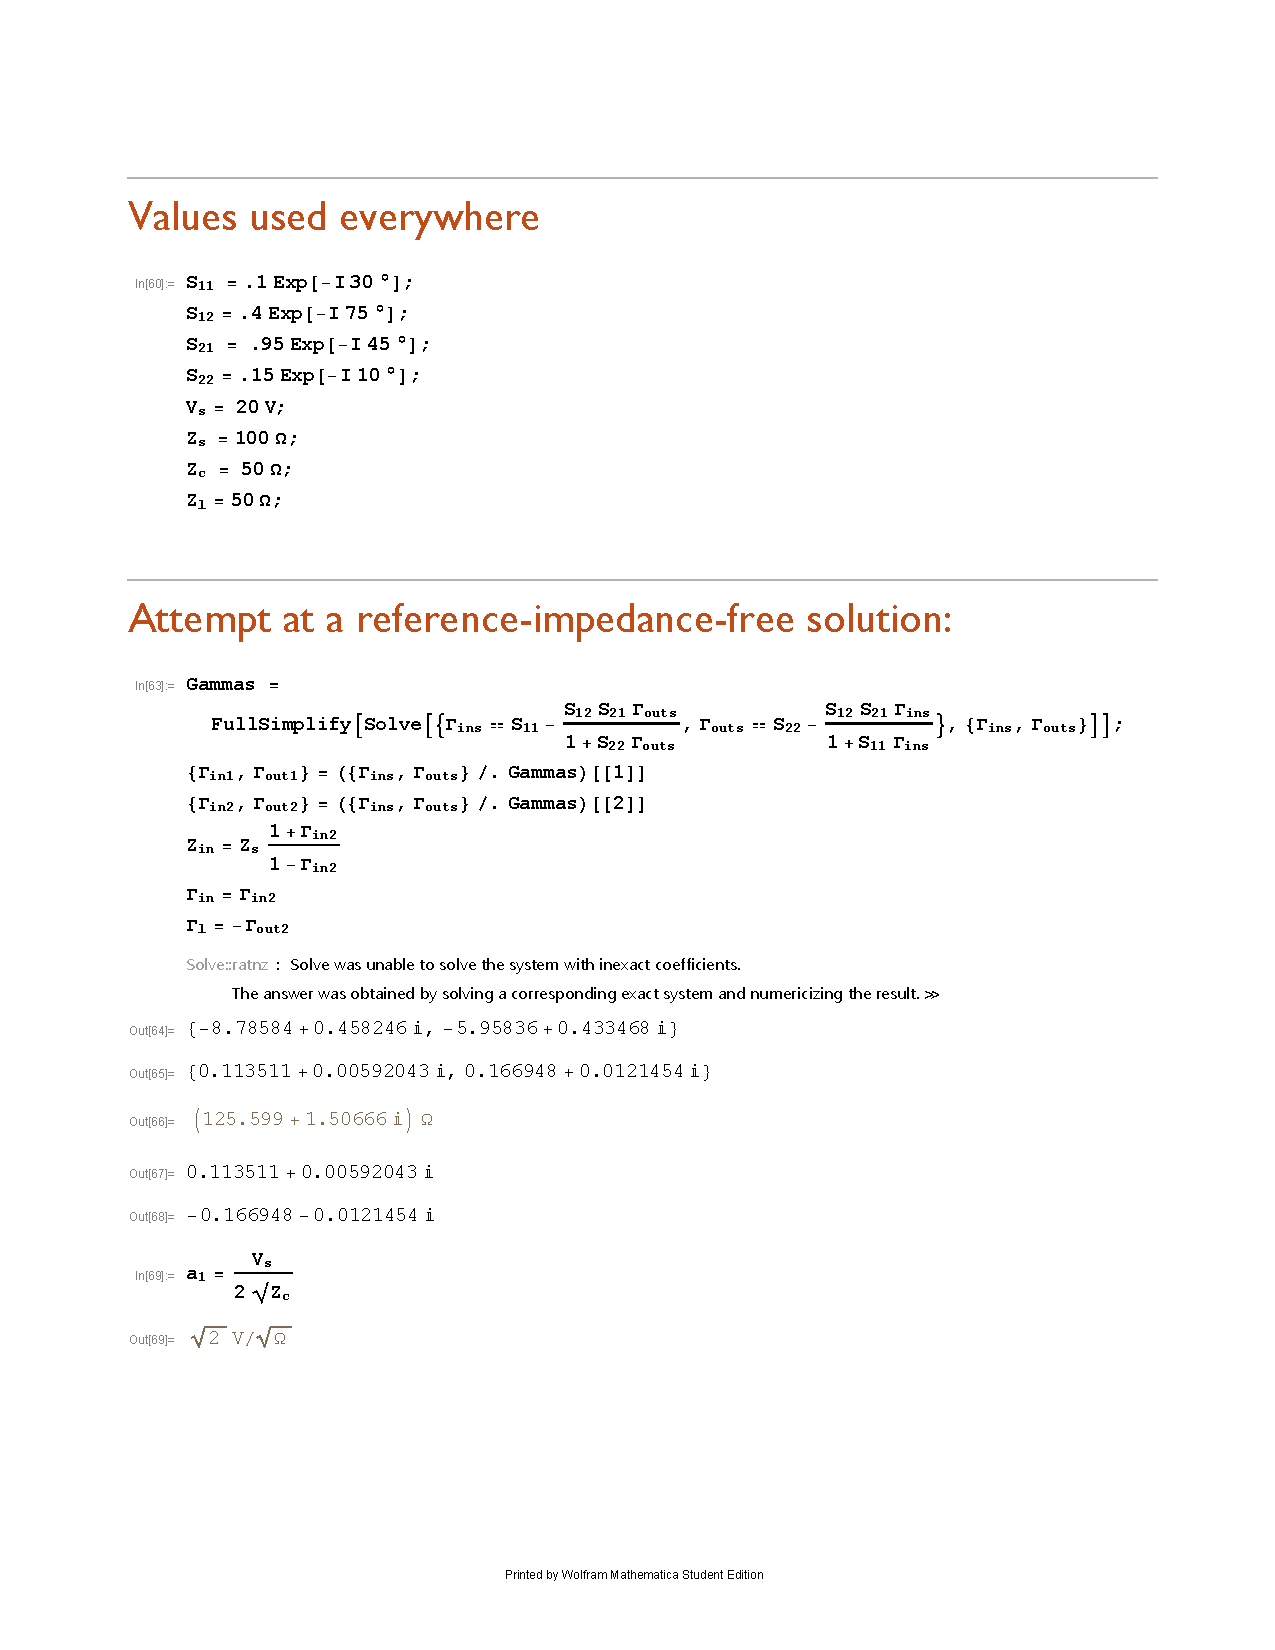
\includepdf[pagecommand={\section{Problem 1
Appendix}\subsection{Mathematica}},scale=.9,pages=1,clip,trim=0cm 5cm 0cm 3cm]{res/Mathematica/Problem1.pdf}
\includepdf[scale=.9,pages=2-,clip,trim=2cm 5cm 0cm 2cm]{res/Mathematica/Problem1.pdf}

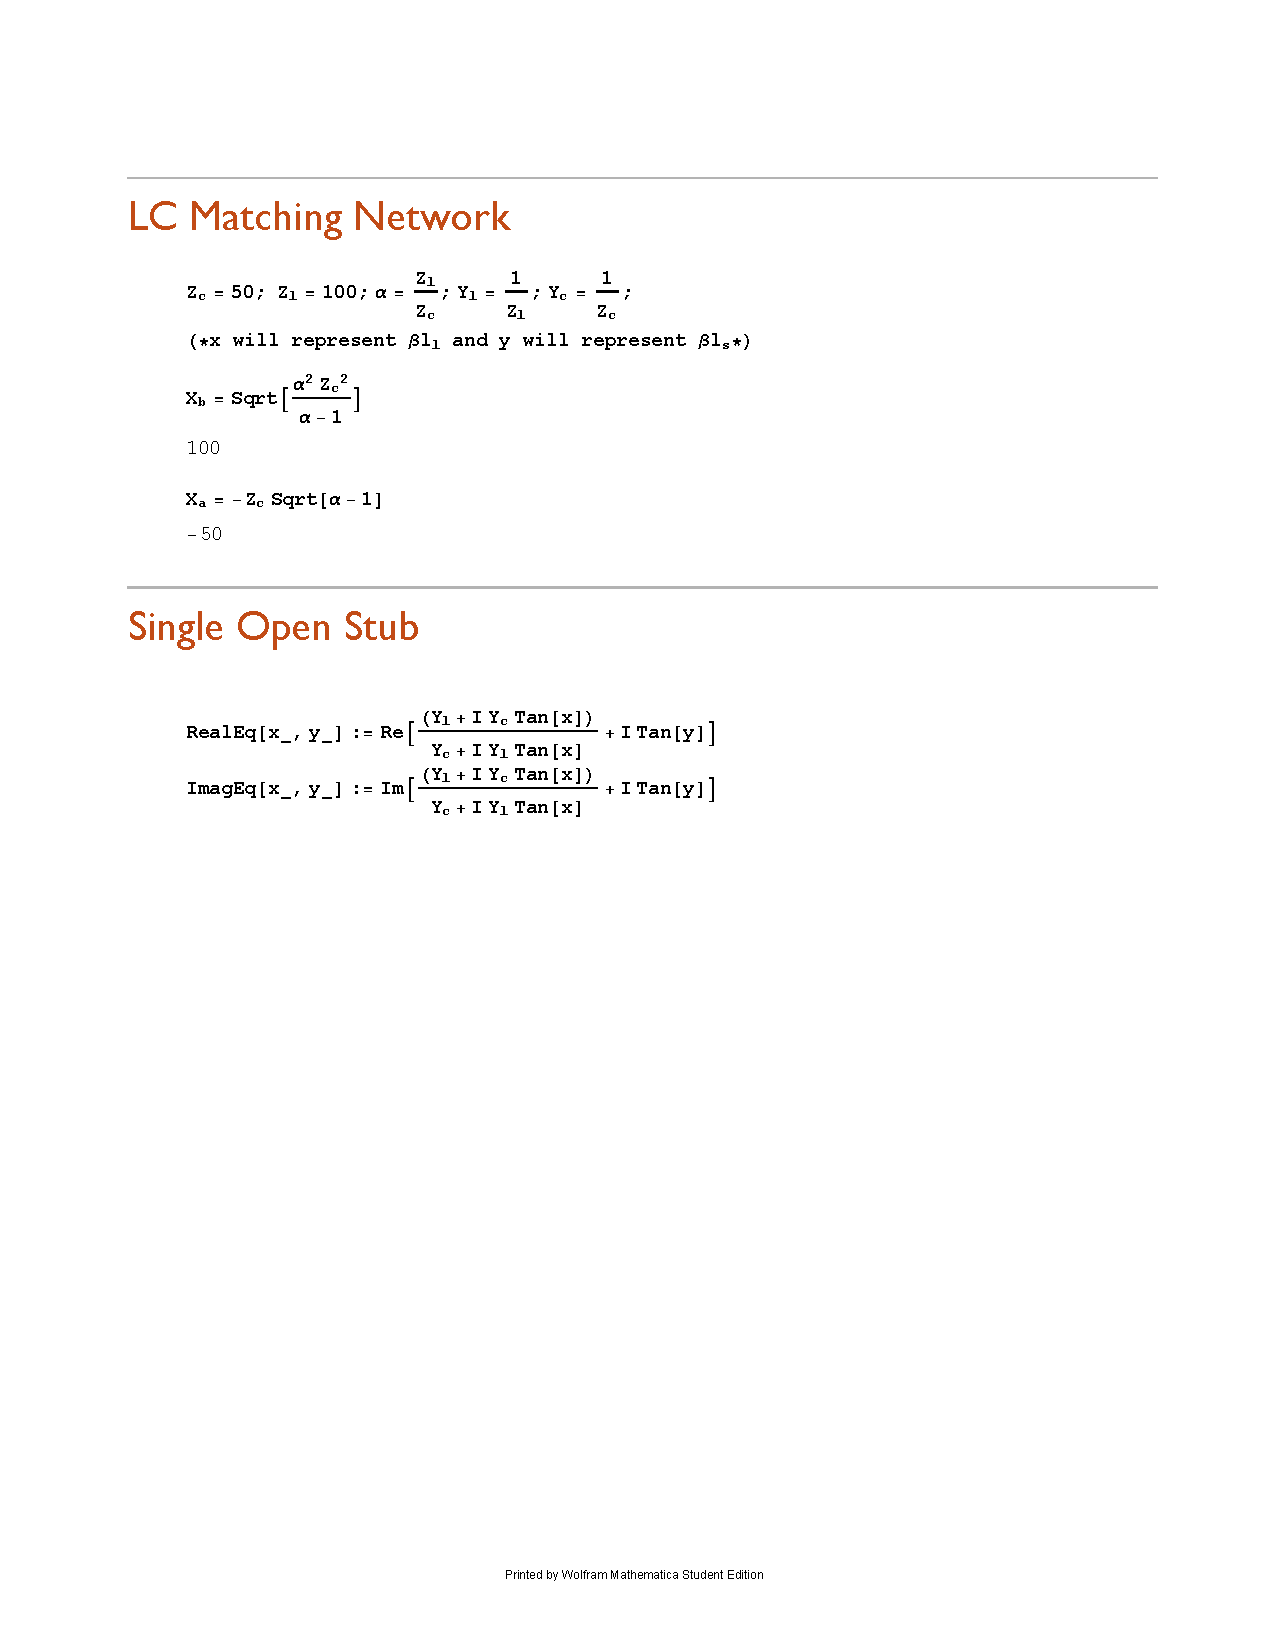
\includepdf[pagecommand={\section{Problem 2 Appendix}\subsection{Mathematica}},scale=.9,pages=1,clip,trim=0cm 5cm 0cm
0cm]{res/Mathematica/Problem2.pdf}
\includepdf[scale=.9,pages=2-,clip,trim=2cm 5cm 0cm 2cm]{res/Mathematica/Problem2.pdf}
\includepdf[scale=.9,pages=2-,clip,trim=2cm 5cm 0cm 2cm]{res/Mathematica/Problem2.pdf}
\subsection{ADS}
\begin{figure}[H]
    \centering
    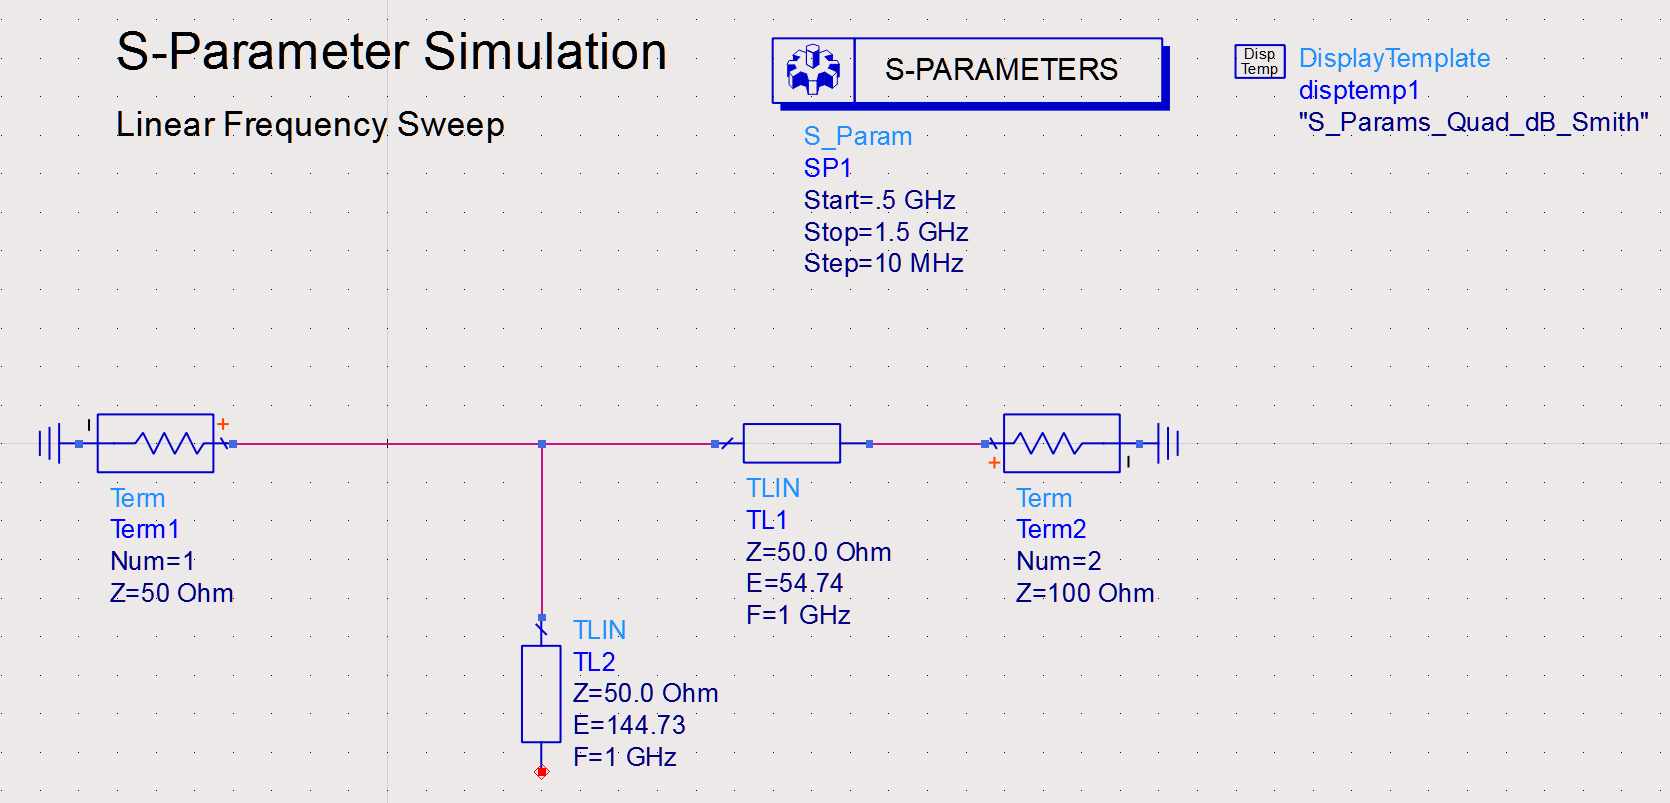
\includegraphics[width=0.8\linewidth]{res/ADS/SingleOpenStubSchematic.png}
    \caption{Schematic for the single open stub tuner.}
    \label{fig:}
\end{figure}
\begin{figure}[H]
    \centering
    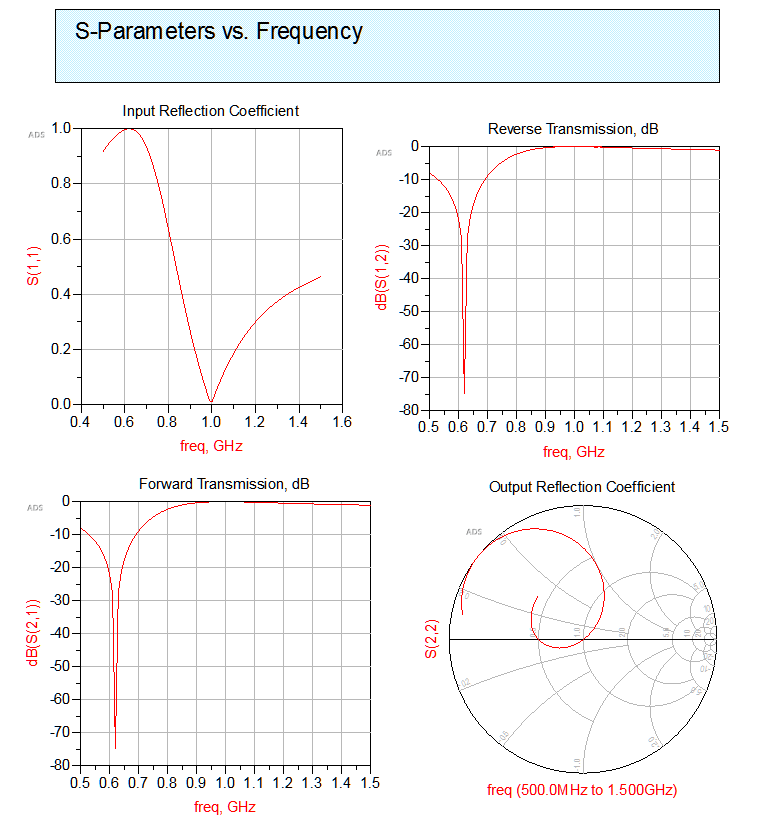
\includegraphics[width=0.8\linewidth]{res/ADS/SingleOpenStub.png}
    \caption{Results for the single open stub tuner.}
    \label{fig:}
\end{figure}

\begin{figure}[H]
    \centering
    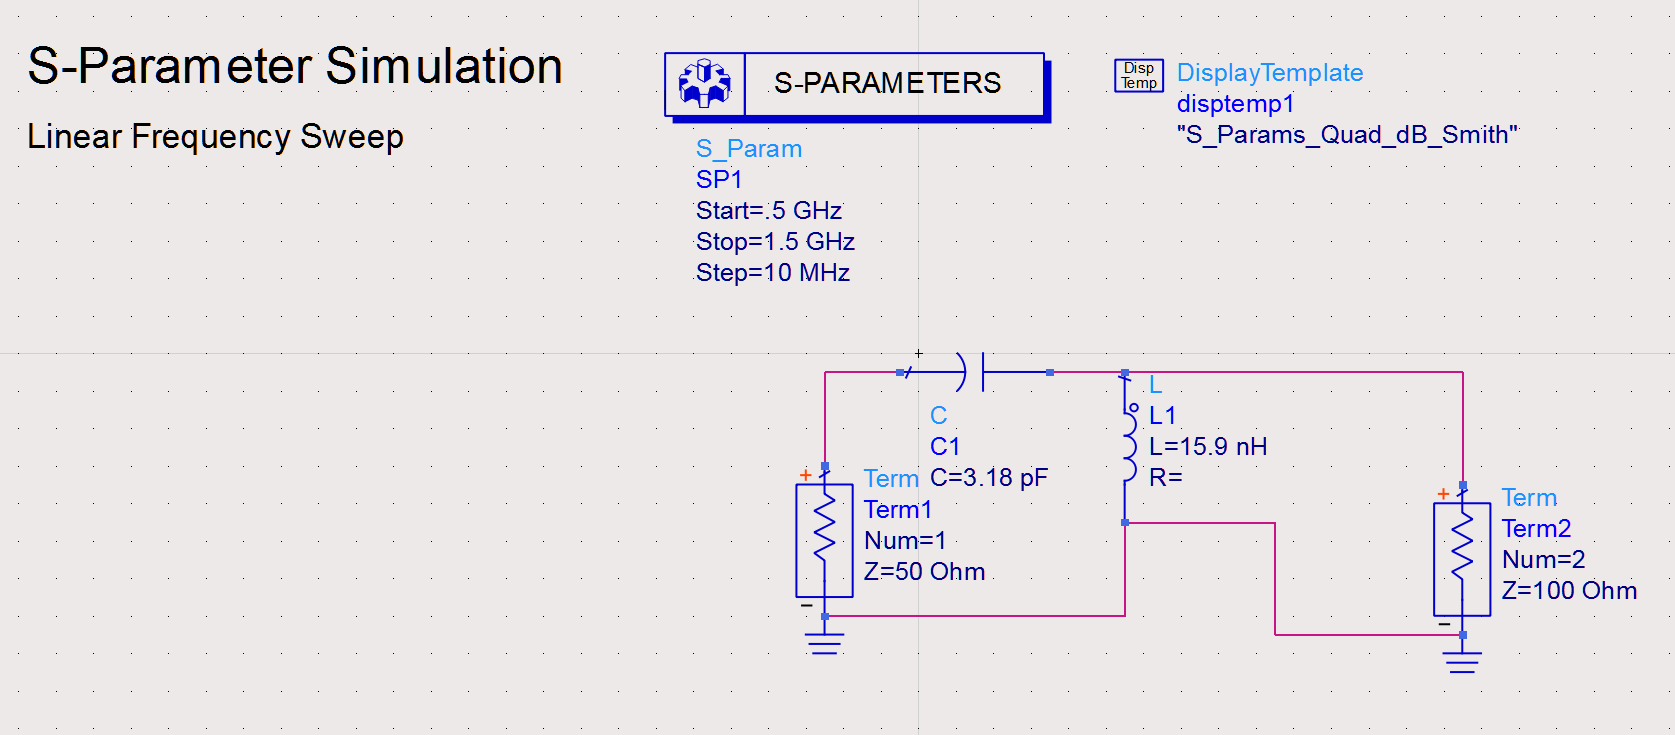
\includegraphics[width=0.8\linewidth]{res/ADS/LCMatchingNetworkSchematic.png}
    \caption{Schematic for the LC Matching Network.}
    \label{fig:}
\end{figure}
\begin{figure}[H]
    \centering
    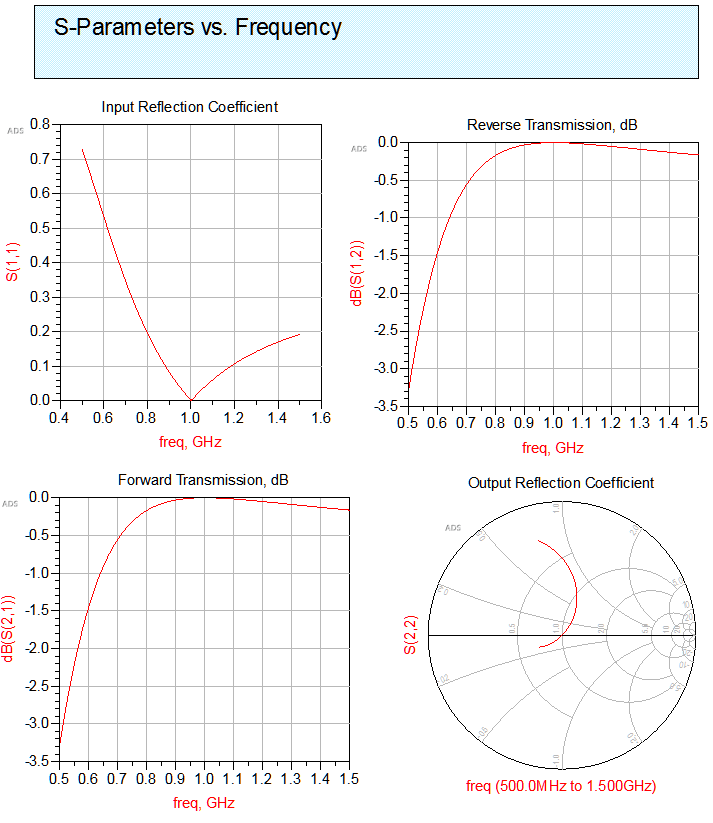
\includegraphics[width=0.8\linewidth]{res/ADS/LCMatchingNetwork.png}
    \caption{Results for the LC Matching Network.}
    \label{fig:}
\end{figure}

\begin{figure}[H]
    \centering
    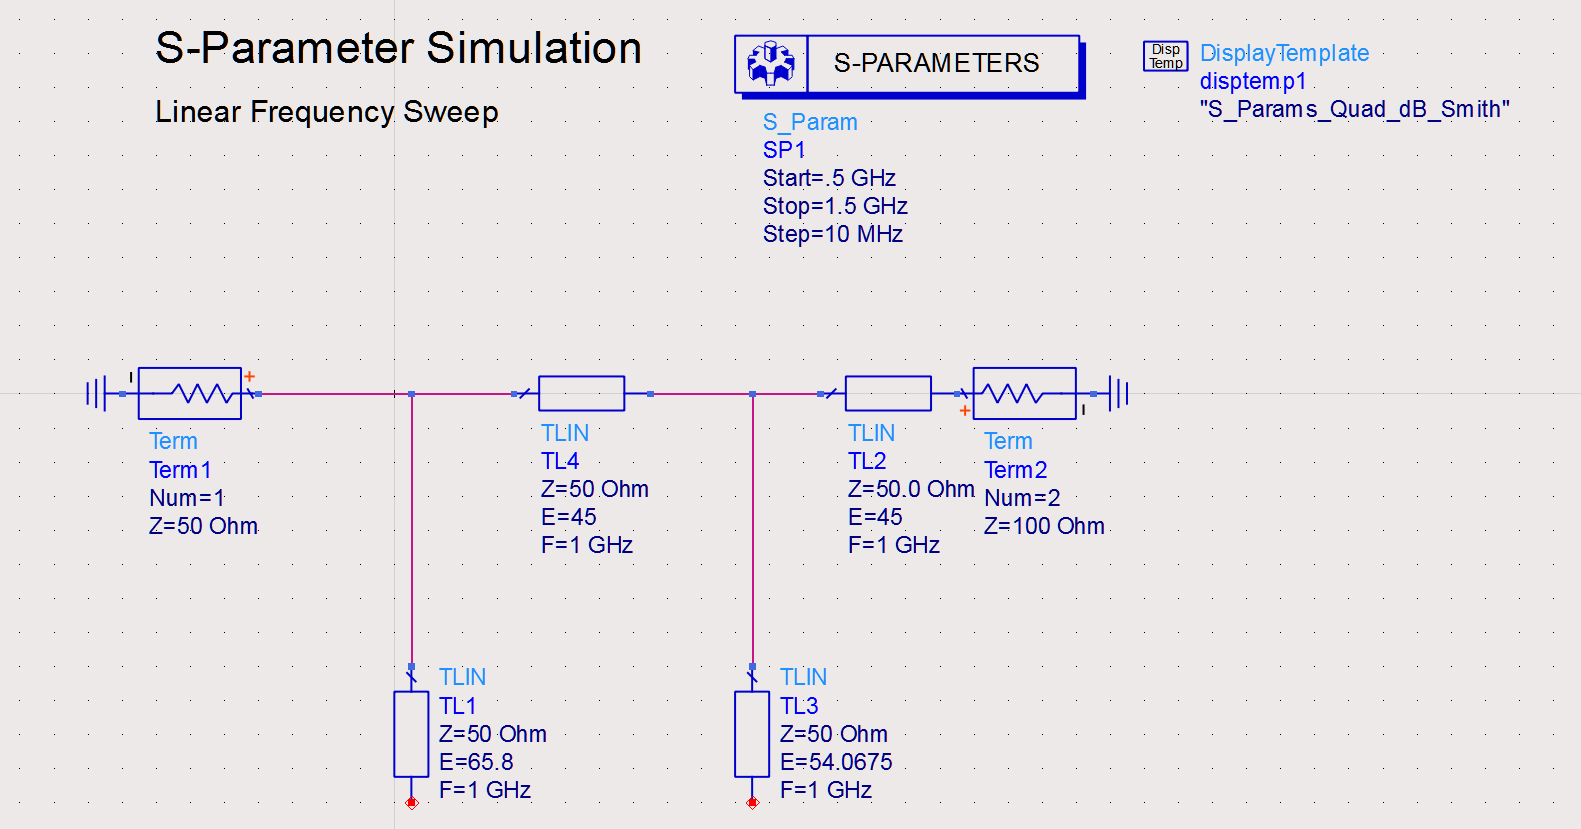
\includegraphics[width=0.8\linewidth]{res/ADS/DoubleOpenStubSchematic.png}
    \caption{Schematic for the double open stub tuner.}
    \label{fig:}
\end{figure}
\begin{figure}[H]
    \centering
    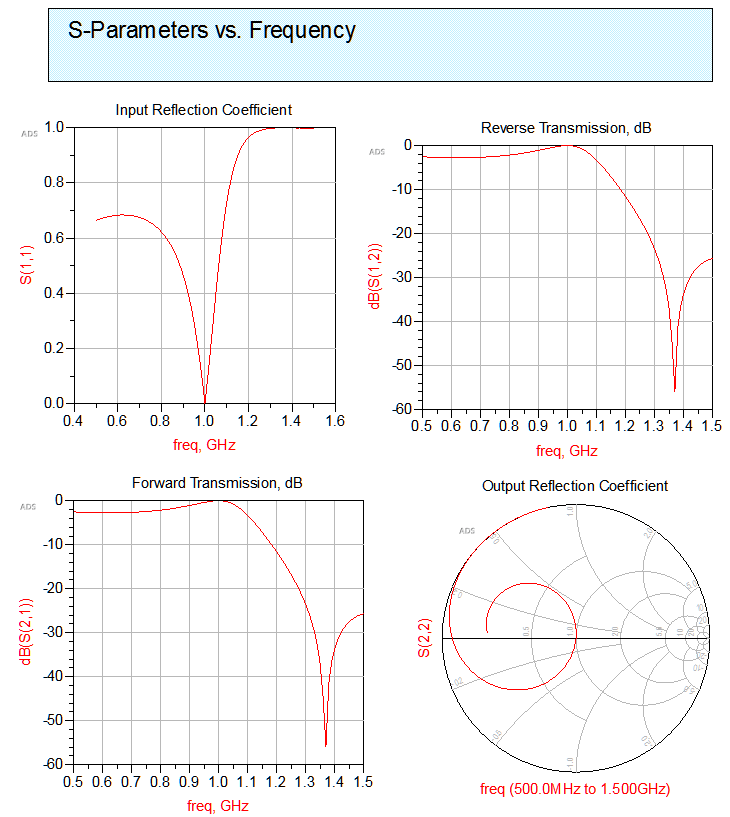
\includegraphics[width=0.8\linewidth]{res/ADS/DoubleOpenStub.png}
    \caption{Results for the double open stub tuner.}
    \label{fig:}
\end{figure}

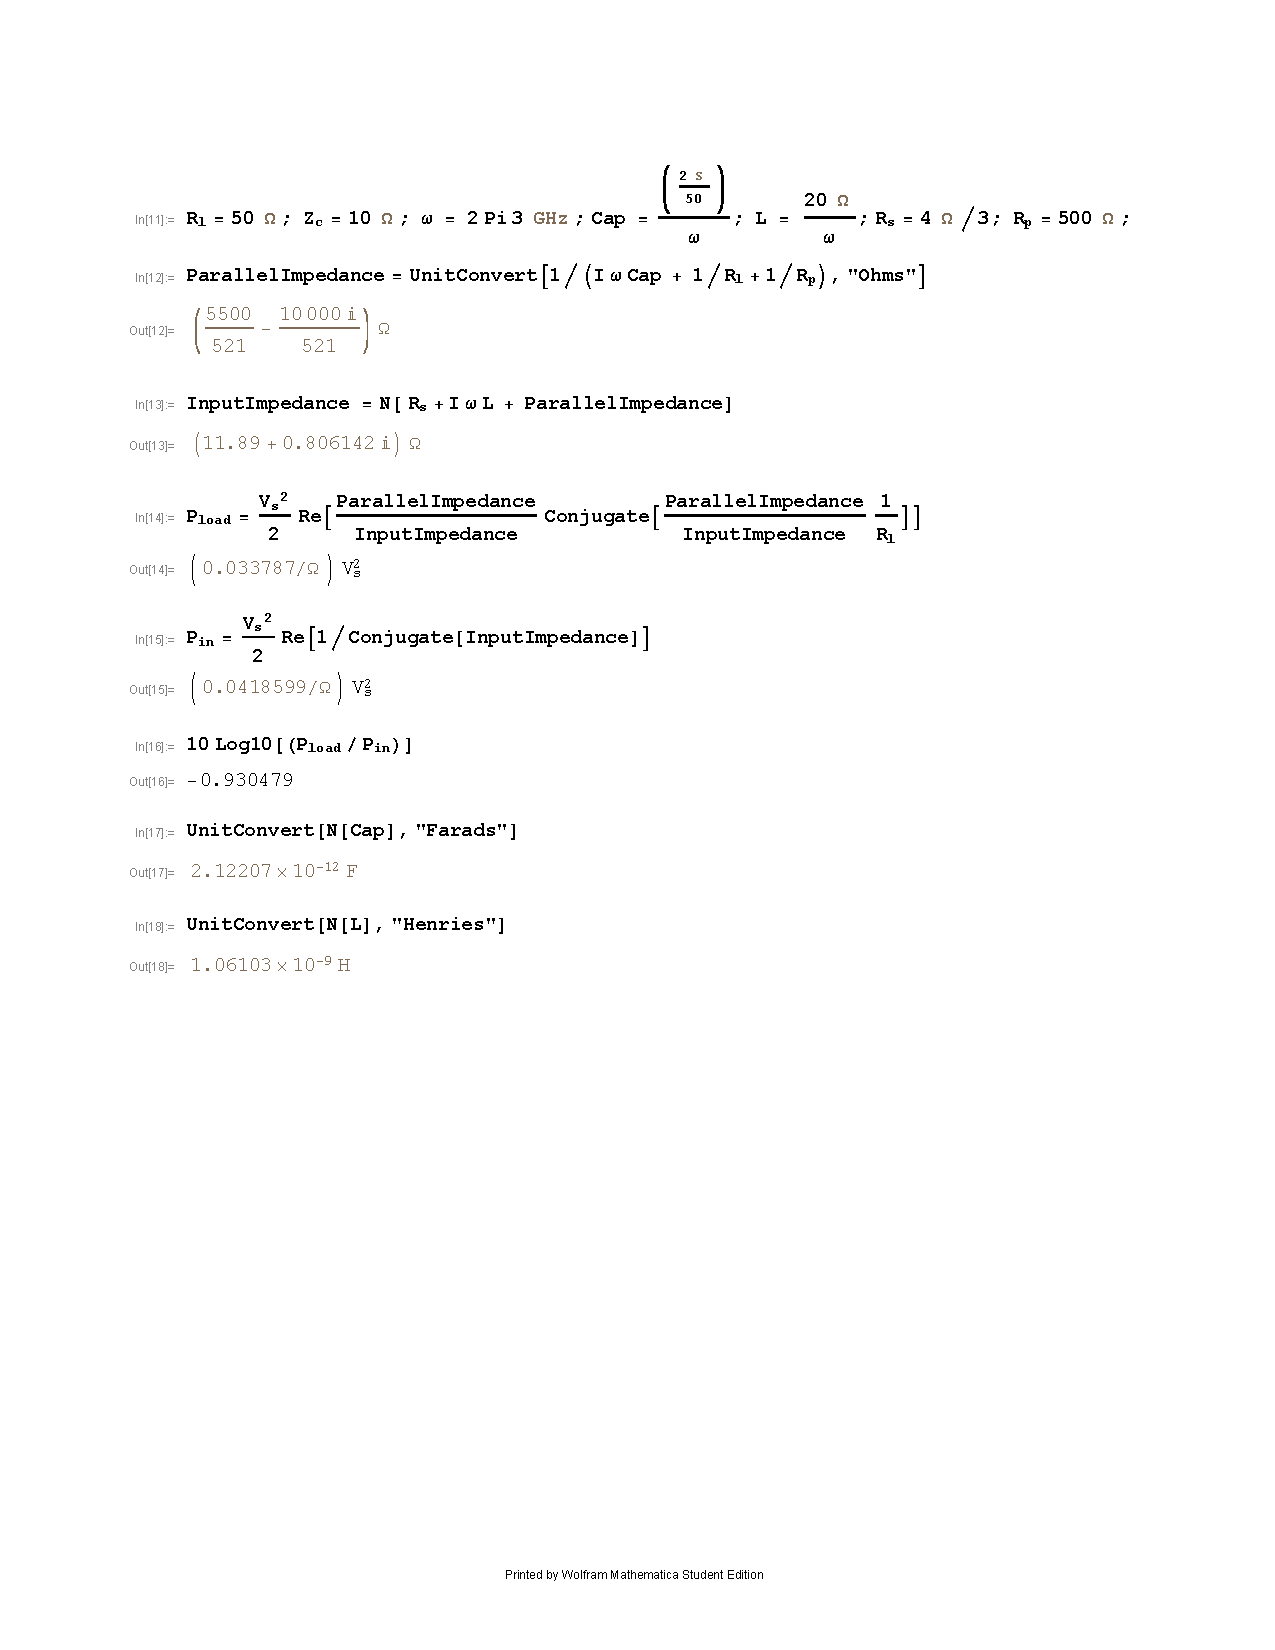
\includepdf[pagecommand=\section{Problem 3 Appendix}\subsection{Mathematica},scale=.9,pages=1,clip,trim=0cm 5cm 0cm 0cm]{res/Mathematica/Problem3.pdf}

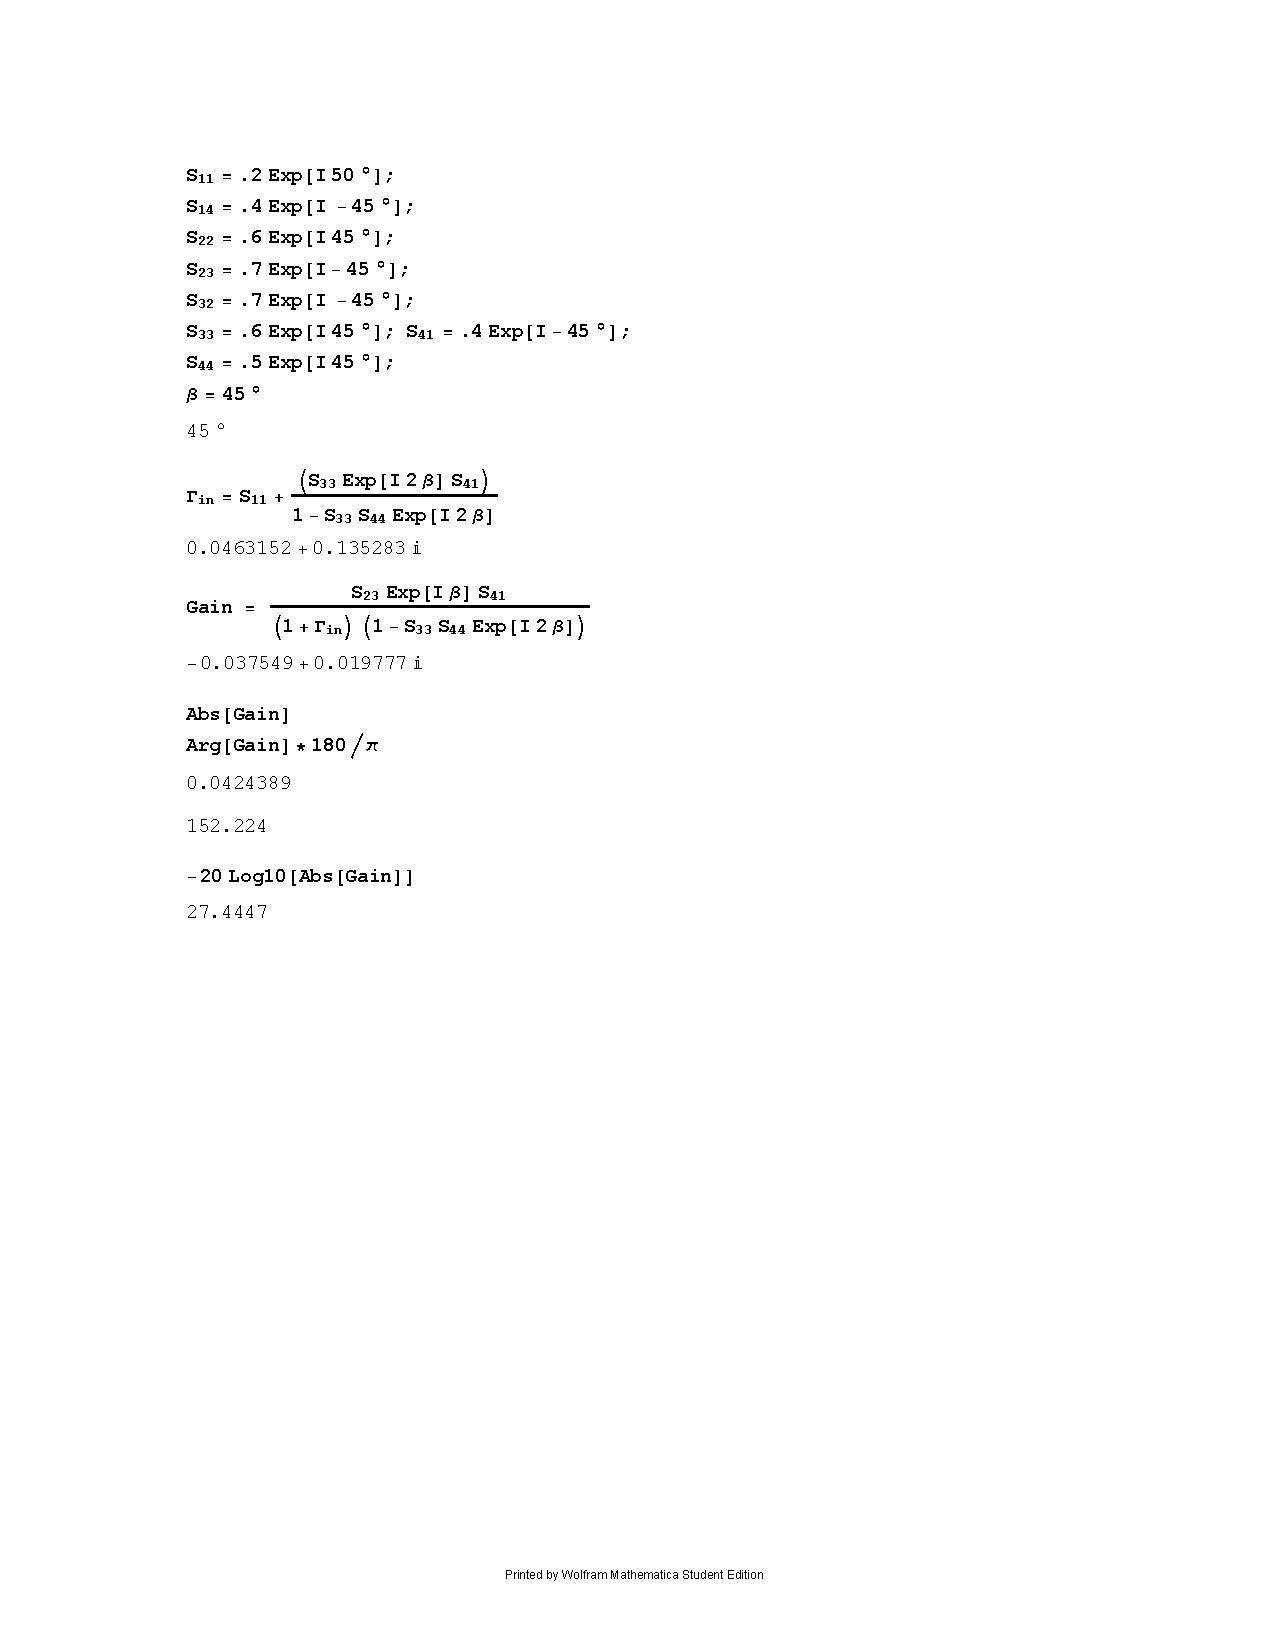
\includepdf[pagecommand=\section{Problem 4 Appendix}\subsection{Mathematica},scale=.9,pages=1,clip,trim=0cm 5cm 0cm 0cm]{res/Mathematica/Problem4.pdf}

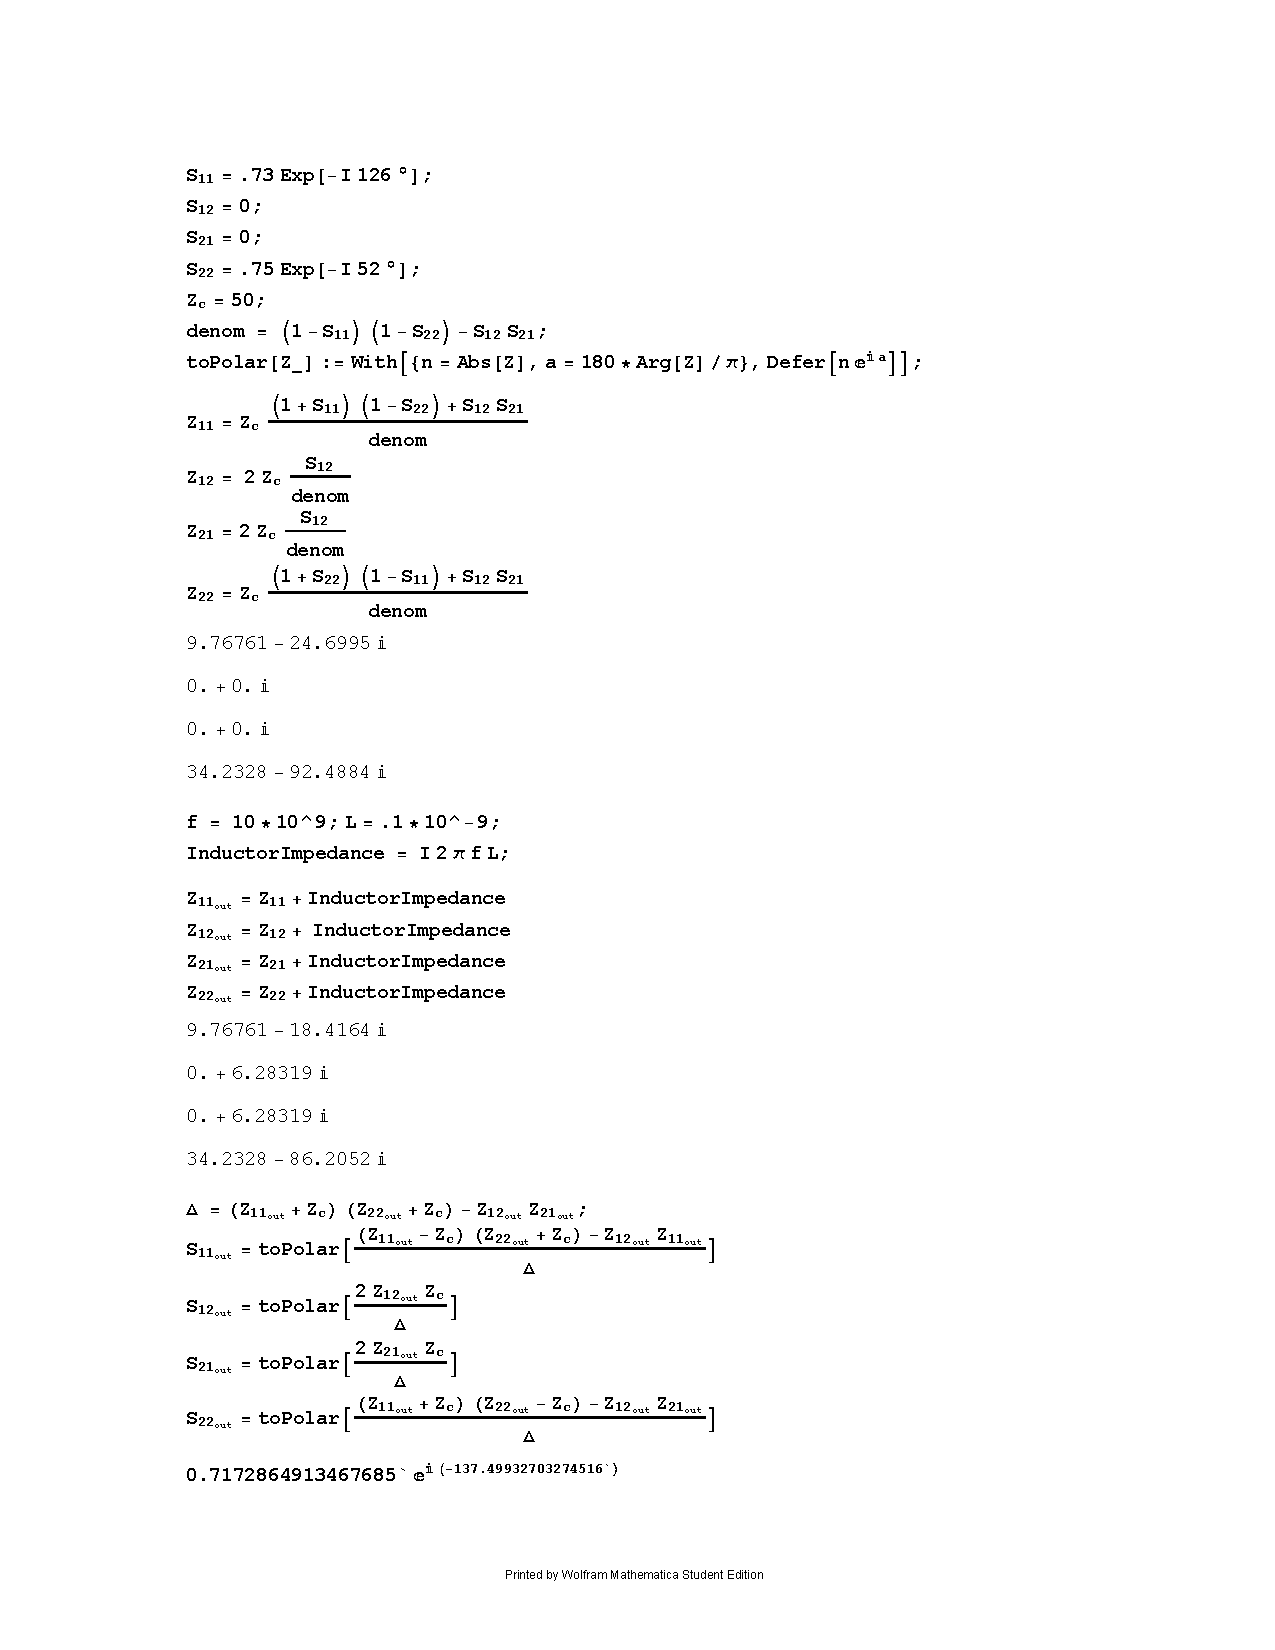
\includepdf[pagecommand={\section{Problem 5 Appendix}\subsection{Mathematica}},scale=.9,pages=1,clip,trim=0cm 5cm 0cm 0cm]{res/Mathematica/Problem5.pdf}
\includepdf[scale=.9,pages=2-,clip,trim=2cm 3cm 0cm 2cm]{res/Mathematica/Problem5.pdf}

\end{document}
